\section{Approach}
\label{sec:approach}

TBD

%We next present our approach for inferring code contracts from method descriptions. Figure~\ref{fig:approach} gives an overview of our approach. Our approach uses a parser, a pre-processor, a text analysis engine, a post-processor, and a code contract generator. The parser accepts the API documents and extracts intermediate contents from the method descriptions. The pre-processor augments the sentences in an intermediate representation with meta-data. The text analysis engine accepts the intermediate representation of the sentences, and then based on our semantic templates, generates specifications in the form of First-Order Logic (FOL) expressions. The post-processor refines the FOL expressions. The code contract generator accepts the FOL expressions and generates code contracts by using a mapping relation to the constructs of the target programming language.
%
%
%
%\begin{figure}
%	\centering
%		\vspace{1mm}		
%		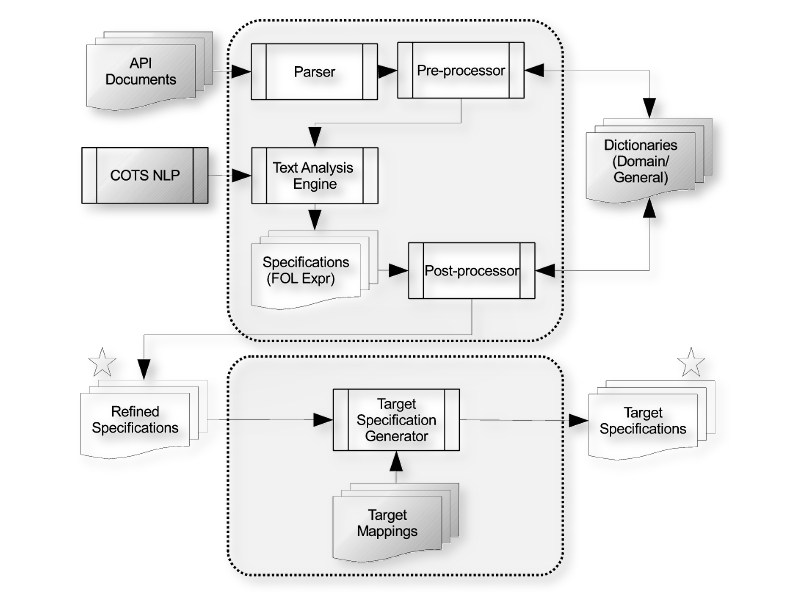
\includegraphics[scale=0.5]{approach.eps}\vspace*{-1ex}
%	\caption{Overview of our approach}\vspace*{-4ex}
%	\label{fig:approach}
%\end{figure}
%
%
%%------------------------------------------------------------------------------------------------
%\vspace*{-1ex}
%\subsection{Parser}
%\label{sub:apip}
%\vspace*{-1ex}
%
%
%Our parser accepts API documents and extracts intermediate contents from the method descriptions. In particular, from the method descriptions, our parser extracts the following contents: (1) \textit{summary description}: the summary of the method; (2) \textit{argument description}: the descriptions of the method's arguments; (3) \textit{return description}: the descriptions of the method's return value; (4) \textit{exception description}: the descriptions of exceptions explicitly thrown by the method; (5) \textit{remark description}: additional descriptions about the functionality of the method.
%
%
%
%%------------------------------------------------------------------------------------------------
%\vspace*{-1ex}
%\subsection{Pre-Processor}
%\label{sub:prep}
%\vspace*{-1ex}
%
%Our pre-processor accepts extracted contents of the method descriptions, and performs three major tasks.
%
%\textbf{Meta-data augmentation}. For each identified method, our pre-processor collects the following meta-data information and associates it with respective sentences: (1) the names and data types of method arguments; (2) the types of the return value and exceptions; (3) the names of the classes, namespaces, and methods. For example, for the method description shown in Figure~\ref{fig:methodAPI}, the meta-data information associated with the sentences in Line 03 is as follows: (1) Sentence Type: Argument Description; (2) Argument Name: \CodeIn{prop\_name}; (3) Argument Type: \CodeIn{String}.
%
%This information is used in code contract generation by substituting the name of the variable with its place-holder and matching a template for code contracts using the data type of the variable. In particular, the pre-processor uses method signatures and their associated tags for meta-data augmentation. From the method signatures, our approach extracts the name of the method arguments, the data types of the method arguments, and the exceptions thrown by the method.
%
%\textbf{Noun Boosting}. Since our text analysis engine uses the Parts-Of-Speech (POS) tags provided by a POS-tagger, the accuracy of the inferred specifications is dependent on the accuracy of the POS-tagger. However, there are specific words that represent nouns in the context of programs, in contrast to adjectives or verbs in the context of general linguistics. For example, consider the statement \textit{``This method also returns false if path is null''}. In this sentence, ``false'' and ``null'' should be treated as nouns since they are constructs of programming languages, but a typical POS tagger would incorrectly classify them as adjectives.
%
%Our pre-processor identifies these words from the sentences based on a domain specific dictionary, and thus forces the underlying POS tagger to identify them as nouns. In particular, our pre-processor uses a predefined list of words for noun boosting. We manually collected these words by looking into the method descriptions in the \CodeIn{Data} class of the Facebook API and the \CodeIn{Path} class of the .NET Framework API. A list of these words is available on our project website.
%
%
%%\begin{figure}
%%	\centering
%%		\includegraphics[scale=0.35, trim=300 100 300 200]{FileMod1.eps}
%%	\caption{An example of NOUN tagging}
%%	\label{fig:sentencetagging1}
%%\end{figure}
%
%	
%
%%Figure~\ref{fig:sentencetagging1} shows the tagged sentence after noun boosting. In the tagged sentence, the NNS tag means singular nouns. 
%
%\textbf{Programming Constructs and Jargon Handling}. In English grammar, the ``.'' character represents the end of a sentence. However, in programming languages,  the ``.''  character is used as a separator character as well. For example, in the \CodeIn{Facebook.Data} namespace, the ``.'' character represents that the \CodeIn{Facebook.Data} namespace exists within the \CodeIn{Facebook} namespace. Our pre-processor identifies these separators, and replaces ``.'' with ``\_''. For example, \CodeIn{"Facebook.Data"} is replaced with \CodeIn{"Facebook\_Data"}.
%
%Additionally, developers tend to use abbreviations for specific words (e.g., max. for maximum and min. for minimum). Our pre-processor identifies these words, and replaces abbreviations with their full names. For example, ``max.'' is replaced with ``maximum''.
%
%These techniques increase the accuracy of the underlying POS tagger, and thus increase the accuracy of our text analysis engine. Furthermore, our pre-processor maintains mapping relations of the place-holder words from the programming language constructs to the original words and locations, and these relations are used by our post-processor later to infer specifications.
%
%Methods and namespaces have a well-defined lexical structure in a programming language. Our pre-processor uses this structural information, and builds regular expressions to identify these words. For handling jargons and abbreviations such as ``max.'', we manually built a list of such words. In future work, we plan to adapt Hill et al.'s technique~\cite{Hill2008} to generate the list automatically.
%
%Although a POS tagger can be retrained to achieve these pre-processing steps, we prefer annotations to make our approach independent of any specific NLP infrastructure, thus ensuring interoperability with various POS taggers.
%
%\vspace*{-1ex}
%\subsection{Text Analysis Engine}
%\label{sub:nlpp}
%\vspace*{-1ex}
%
%
%
%\begin{table*}%
%\centering
%\vspace{2mm}
%\caption{Categories of Shallow Parsing Semantic Templates.}\vspace*{-2ex}
%\begin{tabular}{|r|l|l|l|}
%\hline
%  
%  &Name											&Example																			&Description\\ \hline	\hline		
%%-------------------------------------- END HEADER ------------------------------------------------
%1.&Predicate (Name)					&The (path)$_{subject}$ (can not be)$_{verb}$ 			&The subject and object form the terms of the		\\
%  &													&null$_{object}$																		&predicate represented by verb.									\\ \hline	
%2.&Conditional followed or	&If (path does not have extension)$_{conditional}$,	&The subject-verb-object forms specification		\\
%  &preceded nominal 				&(GetExtension)$_{subject}$ (returns)$_{verb}$ 			&as described in row 1, which is true when the	\\
%  &predicate								&(System.String.Empty)$_{object}$										&condition highlighted by $conditional$ is true.\\
%  & 												&																										&The condition is further resolved using one of	\\
%  &													&																										&the templates.																	\\  \hline	
%3.&Prepositional predicate	&(Path)$_{subject}$ (is)$_{verb}$ (not null  				&The verb forms the partial predicate and the subject\\
%  &													&or empty String)$_{preposition}$										&forms one of the terms. The second term 				\\ 		
%  &													&																										&and the remaining of the predicate are extracted\\
%  &													&																										&by resolving the preposition.									\\  \hline
%4.&Transitive predicate	 		&(Name)$_{subject}$ (is)$_{verb}$ a (valid , 				&The sentence is broken down into two sentences.\\  			
%  &													&identifier)$_{object-subject}$, which (is no 			&The first sentence ends with the phrase labeled \\
%  &													&longer than 32 characters)$_{clause}$							&$_{object-subject}$, and the second sentence begins\\
%  &													&																										&with the phrase labeled $_{object-subject}$. Each sentence\\
%  &													&																										&is further resolved and the resulting specifications\\
%  &													&																										&are joined using the logical AND operator.\\ \hline
%
%\end{tabular}
%
%%\footnotetext[1]{Anonymous read count in the year 2009}
%\vspace*{-3ex}
%\label{tab:pattern}
%\end{table*}
%
%%The text analysis engine parses the pre-processed sentences and tries to infer FOL specifications. The engine uses an NLP technique, called shallow parsing~\cite{Branimir2000}. A shallow parser accepts the lexical tokens generated by an POS tagger and attempts classify the sentence based on defined semantic templates. Shallow parsing is implemented as a sequence of cascading finite state machines. Researches~\cite{Branimir2000,Stickel97,Sinha2009,Gregory99} have shown the efficiency of using finite state machines in different areas of linguistic analysis such as morphological lookup, POS tagging, phrase parsing, and lexical lookup.
%
%%We predefined some templates in our engine, and Table~\ref{tab:pattern} shows four defined semantic templates. Column ``Name'' describes the name of the pattern. Column ``Example'' shows the example when pattern is applied on a sentence. Column ``Description'' shows what is extracted after a pattern is applicable on a sentence.
%
%%In addition to these templates, there are smaller supporting templates to further refine the specifications.  For example, a VERBNOUNLIST pattern associates every term represented by NOUNs present in the list of identified NOUNS to the predicate described in the VERB phrase.
%
%
%
%Our text analysis engine parses pre-processed sentences, and builds specifications in the form of FOL expressions. We chose FOL, since previous research~\cite{Sinha2009,Sinha2010} shows that FOL is an adequate representation for natural language analysis. 
%
%We first use a POS tagger to annotate POS tags in a sentence. We then use an NLP technique, called shallow parsing~\cite{Branimir2000}. A shallow parser accepts the lexical tokens generated by the POS tagger and attempts to classify sentences based on pre-defined semantic templates. Shallow parsing is implemented as a sequence of cascading finite state machines. Research~\cite{Branimir2000,Stickel97,Sinha2009,Gregory99} has shown the effectiveness of using finite state machines in different areas of linguistic analysis such as morphological lookup, POS tagging, phrase parsing, and lexical lookup.
%
% Table~\ref{tab:pattern} shows frequently used semantic templates for identification of specifications. Column ``Description'' describes what is inferred from the sentence if a semantic pattern holds. For example, for the template described in the first row in Table~\ref{tab:pattern}, the FOL expression is constructed as \textit{\textbf{can not be} (path, null)}, where ``path'' and ``null'' are terms to the predicate ``can not be''. The specification is interpreted as: ``can not be'' predicate should be evaluated to be true over terms ``path'' and ``null''.  
%	
%As another example, our text analysis engine uses the semantic pattern, \textit{transitive predicate}, described in the fourth row in Table~\ref{tab:pattern} to analyze the sentence in Line 3 of Figure~\ref{fig:methodAPI}. Figure~\ref{fig:NLPSPEC} shows the graphical FOL expression. Each internal node (shaded grey) represents a predicate and the children of these nodes represent the terms to that predicate.
%
%We implemented a configurable infrastructure to accept a POS tagger to annotate a sentence with POS tags. In particular, for our evaluation, we used the Stanford Parser~\cite{SNLP}, which is a natural language parser to work out the grammatical structure of sentences. The Stanford Parser parses a natural language sentence and determines POS tags associated with different words/phrases. We also implemented a generic and extensible framework that accepts semantic patterns based on the functions of POS tags and converts them into a series of cascading FSMs. Once POS tags have been determined by a POS tagger, the sentences along with tags are passed as an input to the shallow parser, which generate FOL expressions based on the FSMs.
%
%\begin{figure}
%	\centering
%		\includegraphics[scale=0.4, trim=50 0 100 50]{FirstOrderLogic.eps}\vspace*{-4ex}
%	\caption{Specifications in format of FOL expressions extracted by our NLP Parser for \CodeIn{DefineObjectProperty} method in Facebook API}\vspace*{-2ex}
%	\label{fig:NLPSPEC}
%\end{figure}
%
%
%\begin{figure}[t]
%\begin{CodeOut}
%\begin{alltt}
%01:/// <summary>
%02: .....
%03:/// <param name=``prop_name''> This name
%\hspace*{0.2in}needs to be a valid identifier, which
%\hspace*{0.2in}is no longer than 32 characters, starting
%\hspace*{0.2in}with a letter (a-z) and consisting of only
%\hspace*{0.2in}small letters (a-z) numbers (0-9), and/or
%\hspace*{0.2in}underscores.</param>
%04: .....
%05:\textbf{public void} DefineObjectProperty(\textbf{string}
%\hspace*{0.2in}obj_type, \textbf{string} prop_name,
%\hspace*{0.4in}\textbf{int} prop_type)
%\end{alltt}
%\end{CodeOut}\vspace*{-2ex}
%\caption{\label{fig:methodAPI} The method description of the \CodeIn{DefineObjectProperty} method in Facebook API}\vspace*{-4ex}
%\end{figure}
%
%\vspace*{-1ex}
%\subsection{Post-processor}
%\label{sub:postp}
%\vspace*{-1ex}
%
%Our post-processor accepts the FOL expressions produced by the previous component and performs three types of semantic analysis: removing irrelevant modifiers in predicates, classifying predicates into a semantic class based on domain dictionaries, and augmenting expressions. 
%	
%
%\textbf{Equivalence analysis}. Consider the predicate, \textit{`needs to be'}, in FOL representation shown in Figure~\ref{fig:NLPSPEC}. The words, \textit{``needs to''}, are modal modifiers to the verb \textit{'be'}. Such modal modifiers are identified and eliminated. Furthermore, our post-processor classifies predicates into pre-defined semantic classes based on domain dictionaries. This classification addresses the challenge of inferring semantic equivalence. For instance, the predicate, ``starting with'', in Figure~\ref{fig:NLPSPEC} can also be represented as ``begins with''. Our post-processor identifies and classifies all semantically equivalent predicates into a single category, and thus reduces the effort to individually write mappings for every predicate in inferred FOL expressions even when they represent same the semantic function. We have identified the following seven major semantic categories for predicates: (1) Greater, (2) Lesser, (3) Begin, (4) End, (5) Consist, (6) Equal, and (7) Action with respect to expressions dealing with code contracts. The negative semantic categories are represented using a negation operator preceding the identified semantic class.
%	
%	In the preceding semantic analysis, our post-processor uses an NLP technique called lemmatization~\cite{SNLP1}. Lemmatization involves full morphological analysis to accurately identify the lemma for each word. Extracting lemmas reduces the various operational forms of a word to its root. For example, ``am'', ``are'', and ``is'' are all reduced to ``be''. Once the lemma of a word is identified, our post-processor uses the lemma to query a synonym from the WordNet~\cite{wordnet} database for a suitable replacement. From the implementation perspective, we maintain a list of modifier words to identify and discard them. We have also collected synonyms from WordNet to classify a predicate in one of the semantic classes. If a match is not found, our post-processor places the predicate in the unknown category.
%	
%%\begin{figure}
%%	\centering
%%		\includegraphics[scale=0.4, trim=50 25 100 50]{Synonym.eps}
%%	\caption{Specifications after synonym analysis for DefineObjectProperty method in Facebook API}
%%	\label{fig:synonym}
%%\end{figure}
%	
%\textbf{Intermediate Term Elimination}. The intermediate term elimination attempts to remove intermediate terms, if they are found in the extracted expressions. For example, consider the statement in Line 3 of Figure~\ref{fig:methodAPI}. Here, \CodeIn{Valid Identifier} is used as the intermediate term to establish the \CodeIn{"no longer"} relationship between \CodeIn{"name"} and \CodeIn{"32 characters"}. Since a shallow parser is independent of the semantics of the words used in a sentence, our text analysis engine picks up these intermediate terms as valid arguments to the predicate using them, as shown in Figure~\ref{fig:NLPSPEC}. These terms are of no inherent importance in code contract generation.
%		
%	Our post-processor identifies such terms and eliminates them by replacing their usage with their definition. In particular, our post-processor eliminates intermediate terms by parsing FOL expressions. We specifically watch out for terms that are involved in an equality operator with a variable name followed by the same term being used as an input to another predicate in the representation.
%
%\begin{figure}
%	\centering
%		\includegraphics[scale=0.4, trim=200 50 300 0]{Compaction.eps}
%	\caption{FOL expression after synonym analysis and compaction for the \CodeIn{DefineObjectProperty} method in Facebook API}\vspace*{-2ex}
%	\label{fig:compaction}
%\end{figure}
%
%\textbf{Expression Augmentation}. The sentences in return descriptions and exception descriptions in an API document are often not well written. For example, consider the following sentences:
%
%\begin{enumerate}
%	\item \vspace*{-0.5ex}\textit{``true if path is an absolute path; otherwise false.''}--- the return descriptions for the\CodeIn{IsPathRooted} method in the \CodeIn{Path} class in the C\# .NET Framework. The main subject and verb are missing as in what is true and false.
%	\item \vspace*{-0.5ex}\textit{``If path is null.''}--- one of the exception descriptions repeated in many methods in the \CodeIn{File} class in the C\# .NET Framework. The action is missing as in what happens if the path is null.
%	\item \vspace*{-0.5ex}\textit{``IO error occurs while accessing specified directory.''}--- one of the exception descriptions repeated in many methods in the \CodeIn{Directory} class in the C\# .NET framework. While the sentence describes a code contract, the sentence omits important information in terms under what specific condition the exception is thrown.
%\end{enumerate}
%
%
%
%\algsetup{indent=1em}
%\begin{algorithm}[t!]
%\begin{algorithmic}[1]
%\begin{scriptsize}
%\REQUIRE Expr $e$, Meta-data $d$
%\ENSURE Expr $e'$
%\STATE $Expr\ e'\ =\ e$
%\IF{$(d.description==return)$}
%		\IF{$(e'.root==``\rightarrow") \&\& (e'.right\ is\ variable)$}
%				\STATE $Term\ t = e'.right$
%				\IF{$findType(t)==d.returnType$}
%						\STATE $Predicate\ p=new\ Predicate(``returns")$
%						\STATE $p.term = t$
%						\STATE $e'.right = p$
%				\ENDIF
%		\ENDIF
%\ENDIF
%\IF{$(d.description==exception)$}
%		\IF{$(e'.root==``\rightarrow") \&\& (e'.right\ is\ empty)$}
%				\STATE $Term\ t = d.exception\_name$
%				\STATE $Predicate\ p = new\ Predicate\ (``throw")$
%				\STATE $p.term = t$
%				\STATE $e'.right = p$
%		\ENDIF
%		\IF{$(e'.root !==``\rightarrow")$}
%				\STATE $Term\ t = d.exception\_name$
%				\STATE $Predicate\ p = new\ Predicate\ (``throw")$
%				\STATE $p.term = t$
%				\STATE $Expr\ e'' = new\ Expr(``\rightarrow")$
%				\STATE $e''.left = e'$
%				\STATE $e''.right = p$
%				\STATE $e' = e''$
%		\ENDIF
%\ENDIF
%\RETURN $e'$
%\end{scriptsize}
%\end{algorithmic}
%\caption{Expression Augmentation generator}
%\label{alg:SPECAUG}
%\end{algorithm}
%
%\vspace*{-1ex}
%Our expression augmentation attempts to augment these expressions. In particular, for each method, we use meta-data collected in the pre-processor augment to complete the FOL expressions involving return and exception descriptions. Here, we propose Algorithm~\ref{alg:SPECAUG} to achieve our expression augmentation. The algorithm accepts an FOL expression and the meta-data of a sentence. The algorithm returns an augmented expression if successful, and otherwise returns the original expression. The algorithm first checks whether the expression corresponds to a return description statement (Line 2). If the expression is a conditional expression and the right hand side of the expression is a variable term, the algorithm checks whether the type of the variable matches the return type described in the meta-data. Literals, `true', and `false', are identified as boolean; `numeric values' are identified as numeric that matches integer, float, and double. If a match is found, we construct the right hand side of the original predicate as \textbf{returns}.
%
%For the descriptions of exceptions, our expression augmentation does a similar check except that there is no need to match the type of a variable term. We construct the predicate as \textbf{throws}. Additionally, for the expressions in exception descriptions where no conditional expression is identified, we explicitly construct a conditional FOL expression (Line 23-25) and associate the  expression to the left hand side and  the throws predicate to the right hand side.
%
%
%
%
%\vspace*{-2ex}
%\subsection{Code Contract Generator}
%\label{sub:ccg}
%\vspace*{-1ex}
%
%Our code-contract generator generates code contracts from the extracted FOL expressions. The generator uses the predefined mapping of semantic classes of the predicates to the programming constructs to produce valid code contracts. Our current implementation supports the mapping relations for the \CodeIn{String} class, \CodeIn{Integer} class, \CodeIn{null} checks, \CodeIn{return} and \CodeIn{throws} constructs. With more mapping relations, our generator can easily produce code contracts involving complex objects.
%
%
%For example, consider the FOL expression in Figure~\ref{fig:compaction}. The ``greater'' predicate is mapped to the \CodeIn{length} method of the \CodeIn{String} class. Thus, the resulting code contract is \CodeIn{requires(!(name.length()$>$32))}. In contrast, ``begins'' is mapped to the \CodeIn{startswith} and \CodeIn{substring(0,1)} methods of the \CodeIn{String} class. Our generator resolves which methods to choose by taking into account the argument for the method. If the argument is a character (characterized by a single character in quotes) or string (characterized by a string in quotes), our generator uses the \CodeIn{startswith} method, and if the argument is a range (characterized by expression `a--z'), our generator uses the \CodeIn{substring(0,1)} method by converting the range to a regular expression. Thus, the final contract is \CodeIn{requires(name.substring(0, 1).matches("[a-z]+"))}.
%
%\begin{figure}
%\vspace{2mm}
%\begin{CodeOut}
%\begin{alltt}
%01:requires(!prop_name.length()>32)
%02:requires(prop_name.substring(0,1).
%\hspace*{0.2in}matches([a-z]+))
%03:requires(prop_name.matches(([a-z][0-9][_])*))
%\end{alltt}
%\end{CodeOut}\vspace*{-2ex}
%\caption{\label{fig:codecontracts} The inferred specifications for the \CodeIn{prop\_name} variable of the \CodeIn{DefineObjectProperty} method in Facebook API}\vspace*{-6ex}
%\end{figure}}